\chapter{Taxiway design}
	
	\section{Introduction}
	\paragraph{}The aim of the taxiways is to link the different parts of the airport such as the different runways, the terminal, hangars or the parking lot. Several factors must be taken into account when designing this part of the airside; it goes without saying that this design must make the operations easy, efficient and must minimise the total amount of crosses in the flows and in the traffic.
	
	\section{Taxiway's width}
	\paragraph{}OACI’s Annex 14 states that, depending of the code letter, the width must be, at least:
	
	\begin{table}[htb]
		\centering
		\begin{tabular}{ll p{5cm}}
			\toprule[2pt]
			Code letter & Taxiway width [m]\\
			\midrule[1pt]
			A & 7,5\\
			B & 10,5 \\
			C & 15\\
			D & 18-23\\
			E & 23\\
			F & 25\\
			\bottomrule[2pt]
		\end{tabular}
		\caption{Taxiway width depending on its code letter.}
		\label{}
	\end{table}
	
	Due to the fact that our airport has 2 different runways, thus, two different code letters. Thus, the international runway will have a taxiway of 23m since its code letter is E and the domestic one will have 17m since its category is C.
	
	\begin{figure}[H]
		\centering
		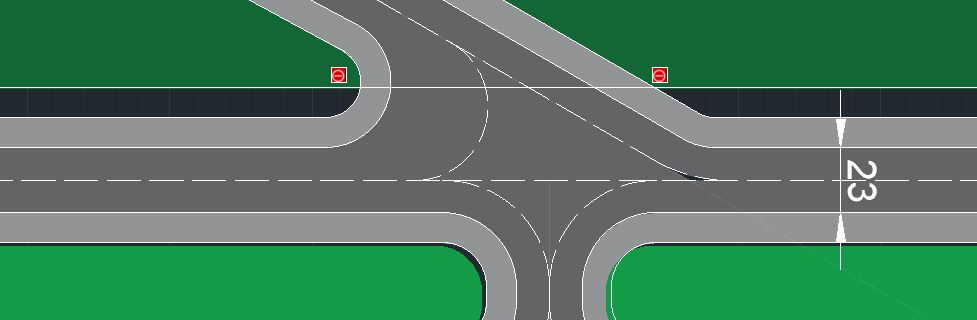
\includegraphics[clip, trim=0.03cm 0cm 0cm 0.03cm, width=0.8\textwidth]{./images/taxiway/width1}
		\caption{Example of the width on the taxiway of runway 1.} %nom de la figura
		\label{} %per denotar una referencia
	\end{figure}

	\begin{figure}[H]
		\centering
		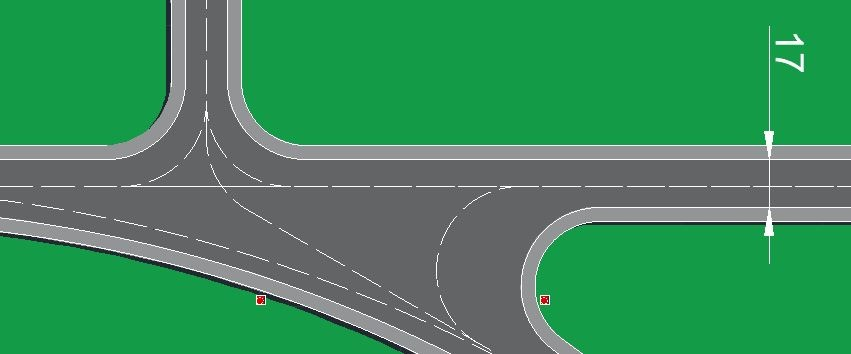
\includegraphics[clip, trim=0.03cm 0cm 0cm 0.03cm, width=0.8\textwidth]{./images/taxiway/width2}
		\caption{Example of the width on the taxiway of runway 2.} %nom de la figura
		\label{} %per denotar una referencia
	\end{figure}
	
	\section{Taxiway's turns}
	\paragraph{}Even though it is recommended that the fewer changes in direction, the better, the Annex 14 stipulates that, for a plane that remains over the taxiway centre line markings, the distance between the outer main wheel and the edge of the taxiway should be, at least:
	
	\begin{table}[htb]
		\centering
		\begin{tabular}{ll p{5cm}}
			\toprule[2pt]
			Code letter & Clearance [m]\\
			\midrule[1pt]
			A & 1,5\\
			B & 2,25 \\
			C & 3-4,5\\
			D & 4,5\\
			E & 4,5\\
			F & 4,5\\
			\bottomrule[2pt]
		\end{tabular}
		\caption{Clearance depending on its code letter.}
		\label{}
	\end{table}

	For the international runway, the clearance will be 4,5m and 3m for the domestic flights runway.
	
	\section{Minimum separation distance}
	\paragraph{}Taking the axis of the taxiway and the axis of the runway or any other taxiway as the reference elements of both paths, under no circumstances should the distance between them be less than the ones shown in table 3.1 in Annex 14 (unless an existing minor distance is proven not to affect negatively the security of the system).
	
	\section{Taxiway's slope}
	\paragraph{}In this section, the taxiway's slope will be boarded, trying to bring solutions in case that the slope can't be changed. 
		\subsection{Longitudinal slope}
		\paragraph{}The longitudinal slope of a taxiway should never exceed:
		
		-	1,5\% if the code letter is C, D, E or F.
		
		-	3\% if the code letter is A or B.
		
		Even though the longitudinal slope has to be tried to be reduced to a minimum, the final longitudinal slope will be 1\% on each runway.
				
		\subsection{Change of the longitudinal slope}
		\paragraph{}If it is not possible to prevent the change of the slope in a taxiway, the transition among them should be a curved surface which curvature should not exceed:
		
		-	1\% for every 30m (radius of curvature approximately 3.000 m) if the code letter is C, D, E or F.
		
		-	1\% for every 25m (radius of curvature approximately 2.500 m) if the code letter is A or B.
	
		Since the longitudinal slope is within the limits established by the ICAO's recommendations, there is not going to be any local change of the longitudinal slope.
		
		\subsection{Visible distance}
		\paragraph{}If changing the slope patterns in a taxiway is not possible, the change in slope should be the one that, from a point situated in:
	
		-	3 m above the taxiway, it could be possible to see a surface of 300 m if the code letter is C, D E or F.
	
		-	2 m above the taxiway, it could be possible to see a surface of 200 m if the code letter is B.
	
		-	1,5 m above the taxiway, it could be possible to see a surface of 150 m if the code letter is A.
	
		\subsection{Transversal slope} 
		\paragraph{}The cross slope of a taxiway, as in runways, should be strong enough to prevent the accumulation of water in its surface, but should never be greater than:
		
		-	1,5\% if the code letter is C, D, E or F.
		
		-	2\% if the code letter is A or B.
		
		The transversal slope selected for both taxiways is 1,5\%.
	
	\section{Taxiway's shoulders}
	\paragraph{}OACI’s Annex 14 recommends that taxiways subordinated to runways with code letter C, D, E or F should be designed with symmetrical margins, in order to make the total width of the taxiway, that is to say, taxiway and margins, greater than:
	
	-	60 m if the code letter is F.
	
	-	44 m if the code letter is E.
	
	-	38 m if the code letter is D.
	
	-	25 m if the code letter is C.
	
	An additional width should be added in curves, unions and intersections.
	
	Following the recommendation shown above, the taxiway's shoulders of runway 1 will be 44m and the taxiway's shoulders of runway 2 will be 27m.
	
	\begin{figure}[H]
		\centering
		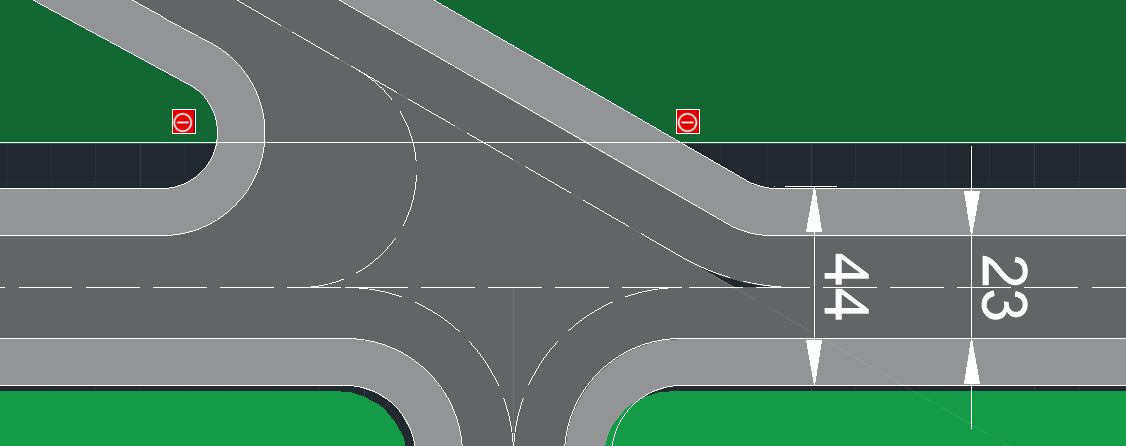
\includegraphics[clip, trim=0.03cm 0cm 0cm 0.03cm, width=0.8\textwidth]{./images/taxiway/shoulders1}
		\caption{Example of the shoulders distance on the taxiway of runway 1.} %nom de la figura
		\label{} %per denotar una referencia
	\end{figure}

	\begin{figure}[H]
		\centering
		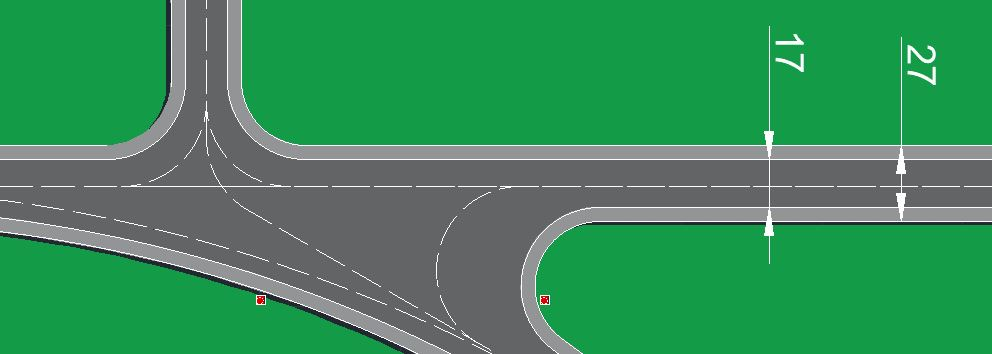
\includegraphics[clip, trim=0.03cm 0cm 0cm 0.03cm, width=0.8\textwidth]{./images/taxiway/shoulders2}
		\caption{Example of the shoulders distance on the taxiway of runway 2.} %nom de la figura
		\label{} %per denotar una referencia
	\end{figure}
	
	\section{Rapid exit taxiways}
		\paragraph{}As a recommendation, a rapid-exit taxiway should be calculated with a turn radius of, at least:
		
		-	550 m if code number 3 or 4.
		
		-	275 m if code number 1 or 2.
		
		In order to make the exit possible with a wet pavement at a speed of;
		
		-	93 km/h if code number 3 or 4.
		
		-	65 km/h if code number 1 or 2.
		
		Moreover, the angle of rapid-exit taxiways should be comprehended between 45\(\degree\) and 25\(\degree\), preferably 30\(\degree\). Rapid-exit taxiways should also include a straight section in order to allow the air plane to reduce its speed. 
		
		